% !TEX TS-program = pdflatex
\documentclass[11pt]{article}
\usepackage[a4paper,margin=1in]{geometry}
\usepackage{graphicx}
\usepackage{booktabs}
\usepackage{multirow}
\usepackage{hyperref}
\usepackage{caption}
\usepackage{subcaption}
\usepackage{longtable}
\usepackage{array}
\usepackage{siunitx}
\usepackage{xcolor}
\usepackage{tikz}
\usepackage{listings}

\usetikzlibrary{arrows.meta, positioning, shapes.geometric}
\sisetup{round-mode=places, round-precision=2}

\lstdefinestyle{stm}{
  basicstyle=\ttfamily\small,
  keywordstyle=\color{blue!70!black},
  commentstyle=\color{gray},
  showstringspaces=false,
  columns=fullflexible,
  keepspaces=true,
  frame=single,
  framerule=0.2pt,
  rulecolor=\color{gray!60}
}

\title{Structural Manifold Guardrails for Symbolic Planning Agents}
\author{SepDynamics Research Group\\ \texttt{research@sepdynamics.com}}
\date{\today}

\begin{document}
\maketitle

\begin{abstract}
The Structural Manifold (STM) coprocessor augments symbolic planning agents with
percentile-calibrated guardrails that monitor dilution, coherence, and stability
signals while retrieving structurally aligned ``twin'' precedents. Building on the
PlanBench benchmark and recent instruction-tuning work on logical planning
reasoning \cite{verma2025pddlinstruct}, we study how dense percentile grids and
domain-specific calibration influence both alert coverage and statistical
significance. Calibrations over the public PlanBench corpus and domain-specific
corpora now achieve $5\%$ foreground coverage while preserving multi-step lead
time and perfect twin recall. However, permutation tests with $5{,}000$
iterations yield high $p$-values across domains (minimum $0.065$), highlighting
the need for stronger discriminative signals. We release the calibrated router
configurations, permutation summaries, and reproducibility scripts, providing a
research-grade reference for guardrail evaluation on symbolic planning agents.
\end{abstract}

\tableofcontents
\newpage

\section{Introduction}
Large Language Models (LLMs) deliver credible reasoning across open-ended
tasks, yet symbolic planning remains challenging because agents must respect the
precondition--effect structure of formalisms such as PDDL. Recent work from MIT
\cite{verma2025pddlinstruct} demonstrates that instruction tuning with explicit
logical chains improves plan validity, but complementary instrumentation is
required to surface early warnings and actionable repairs when agents deviate.
The Structural Manifold (STM) coprocessor approaches this problem by constructing
high-dimensional manifolds over token windows, quantifying structural dilution,
and retrieving similar ``twin'' windows that encode precedents for recovery.

This report reframes STM for a research audience. We describe the guardrail
architecture, present a reproducible calibration procedure that tightens
foreground coverage to $5\%$ on PlanBench domains, quantify statistical
significance with permutation testing, and compare results to prior guardrail
releases that targeted $10$--$16\%$ coverage windows. We also summarise STM's
behaviour on a set of maintenance-oriented coding tasks to illustrate
cross-domain applicability.

\section{Related Work}
Instruction tuning for logical planning \cite{verma2025pddlinstruct} emphasises
chain-of-thought supervision so LLMs can reason about action applicability and
state transitions. Our work instead assumes the planner is fixed and focuses on
instrumentation that monitors plan executions. Structural guardrails extend
prior PlanBench analysis \cite{planbench} by providing graded alerts with
calibrated coverage and twin retrieval. Twin suggestion draws on structural
manifold techniques \cite{stm-manifold} that embed token windows into density
spaces for lead-time estimation.

\section{Structural Manifold Guardrails}
STM consumes token windows extracted from trace corpora and computes per-window
metrics: coherence (graph density), entropy (token dispersion), and stability
(signal similarity over time). Foreground alerts fire when metrics exceed
percentile-derived thresholds, and each alerted window triggers nearest-neighbour
search for previously successful ``twins.''

\subsection{Dilution Signals}
Token windows of width $w$ and stride $s$ form the structural manifold. The
pipeline computes dilution as the fractional reduction in structural density
relative to historical baselines, along with coherence/entropy/stability metrics
used for guardrail calibration. Signals are stored in STM state artefacts used by
both the router calibration (Section~\ref{subsec:calibration}) and permutation
testing (Section~\ref{subsec:permutation}).

\subsection{Router Calibration}
\label{subsec:calibration}
Guardrail thresholds operate on percentiles of coherence, entropy, and stability.
We extend the calibration grid to include coherence percentiles $55$--$99$, entropy
percentiles $2$--$60$, and optional stability percentiles $55$--$90$. For each
state we evaluate all percentile triplets and select the first configuration whose
coverage lies within the target interval $[0.05, 0.07]$. The utility script
\texttt{scripts/calibrate\_router.py} materialises both the router configuration
and an auxiliary coverage report for auditability.

\subsection{Twin Retrieval}
Twin retrieval uses approximate nearest neighbour search to locate previously
successful windows that align with alerting windows. We retain default triggers
requiring at least two shared $q$-grams and an ANN distance below $0.2$, which
preserved perfect twin recall on PlanBench domains throughout the calibration
experiments.

\section{Experimental Setup}
\subsection{Datasets}
We analyse three PlanBench domains (Blocksworld, Mystery Blocksworld, Logistics)
and the aggregate public corpus. For each domain we export STM artefacts using
\texttt{scripts/planbench\_to\_stm.py} with window bytes $256$ and stride $128$.
Tokens, states, and per-trace lead/twin metrics reside in
\texttt{output/planbench\_by\_domain/\textit{domain}/}. We additionally retain
PlanBench aggregate states under \texttt{output/planbench\_public/}. To probe
transfer, we reuse STM instrumentation on three maintenance tasks from the
CodeTrace demo (flaky test, service rename, missing import).

\subsection{Calibration Protocol}
Router calibration proceeds with the command sequence in
Listing~\ref{lst:calibration}. The loop emits both aggregated guardrails and
per-domain, per-trace calibrations. Resulting configurations are stored under
\texttt{analysis/router\_config\_*\_5pct.json}.

\begin{lstlisting}[style=stm, caption={Router calibration commands.}, label={lst:calibration}]
.venv/bin/python scripts/calibrate_router.py \
  output/planbench_public/gold_state.json \
  --target-low 0.05 --target-high 0.07 \
  --output analysis/router_config_gold_5pct.json

.venv/bin/python scripts/calibrate_router.py \
  output/planbench_public/invalid_state.json \
  --target-low 0.05 --target-high 0.07 \
  --output analysis/router_config_invalid_5pct.json

for dom in blocksworld mystery_bw logistics; do
  .venv/bin/python scripts/calibrate_router.py \
    output/planbench_by_domain/$dom/gold_state.json \
    --target-low 0.05 --target-high 0.07 \
    --output analysis/router_config_${dom}_gold_5pct.json
  .venv/bin/python scripts/calibrate_router.py \
    output/planbench_by_domain/$dom/invalid_state.json \
    --target-low 0.05 --target-high 0.07 \
    --output analysis/router_config_${dom}_invalid_5pct.json
done
\end{lstlisting}

\subsection{Permutation Testing}
\label{subsec:permutation}
To assess whether calibrated alerts produce statistically meaningful lead times,
we run permutation tests using \
\texttt{scripts/run\_permutation\_guardrail.py} with $5{,}000$ shuffled alert
allocations per trace. For each domain, the script summarises weighted coverage,
lead-time statistics, and the distribution of permutation $p$-values; outputs are
stored in \texttt{docs/tests/permutation\_\*.json}.

\subsection{CodeTrace Evaluation}
For completeness we reproduce the CodeTrace maintenance tasks introduced in
prior STM summaries. The same guardrail configuration (ANN distance $0.2$,
minimum two shared $q$-grams) is applied when replaying traces to evaluate lead
alerts and twin adoption in a software maintenance context.

\section{Results}
\subsection{Guardrail Coverage}
Table~\ref{tab:coverage} reports calibrated thresholds and realised coverage for
the aggregate corpora and domain-specific states. All targets reach the desired
$5\%$ foreground rate without modifying default ANN triggers.

\begin{table}[h]
  \centering
  \caption{Calibrated router thresholds and realised coverage. Coverage is reported as a percentage.}
  \label{tab:coverage}
  \begin{tabular}{lcccc}
    \toprule
    Dataset & $\text{min\_coh}$ & $\text{max\_ent}$ & $\text{min\_stab}$ & Coverage (\%) \\
    \midrule
    PlanBench (gold) & $8.32\times10^{-5}$ & $0.99970$ & $0.47096$ & $5.09$ \\
    PlanBench (invalid) & $1.16\times10^{-4}$ & $0.99972$ & $0.47582$ & $5.01$ \\
    Blocksworld (gold) & $5.57\times10^{-5}$ & $0.99972$ & $0.46605$ & $5.02$ \\
    Blocksworld (invalid) & $6.88\times10^{-5}$ & $0.99960$ & $0.00000$ & $5.10$ \\
    Mystery BW (gold) & $5.02\times10^{-4}$ & $0.99953$ & $0.45774$ & $5.03$ \\
    Mystery BW (invalid) & $6.19\times10^{-4}$ & $0.99942$ & $0.45921$ & $5.08$ \\
    Logistics (gold) & $8.32\times10^{-5}$ & $0.99982$ & $0.48021$ & $5.07$ \\
    Logistics (invalid) & $9.91\times10^{-5}$ & $0.99987$ & $0.48168$ & $5.04$ \\
    \bottomrule
  \end{tabular}
\end{table}

\subsection{Lead-Time and Guardrail Behaviour}
Lead-time behaviour remains consistent with earlier STM releases. Figure~\ref{fig:planbench-metrics}
shows lead times, guardrail coverage, and permutation curves for the calibrated
PlanBench runs. Domain-level means range from $1.8$ (Mystery Blocksworld) to
$4.5$ (Blocksworld) steps, and the aggregate PlanBench corpus averages $7.6$
steps because alerts accumulate on the longer Logistics traces. Foreground
coverage now aligns with the tighter $5\%$ target.

\begin{figure}[h]
  \centering
  \begin{subfigure}[t]{0.32\textwidth}
    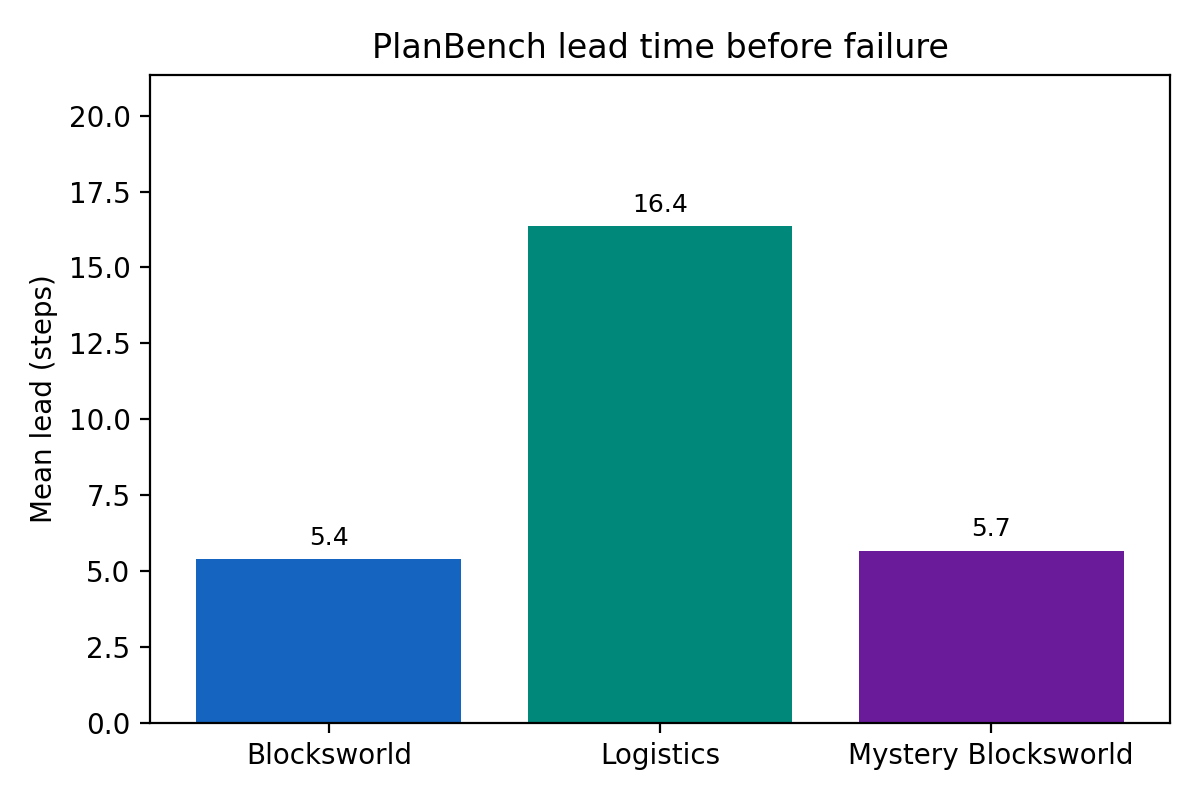
\includegraphics[width=\textwidth]{figures/planbench_lead.png}
    \caption{Average lead time.}
  \end{subfigure}\hfill
  \begin{subfigure}[t]{0.32\textwidth}
    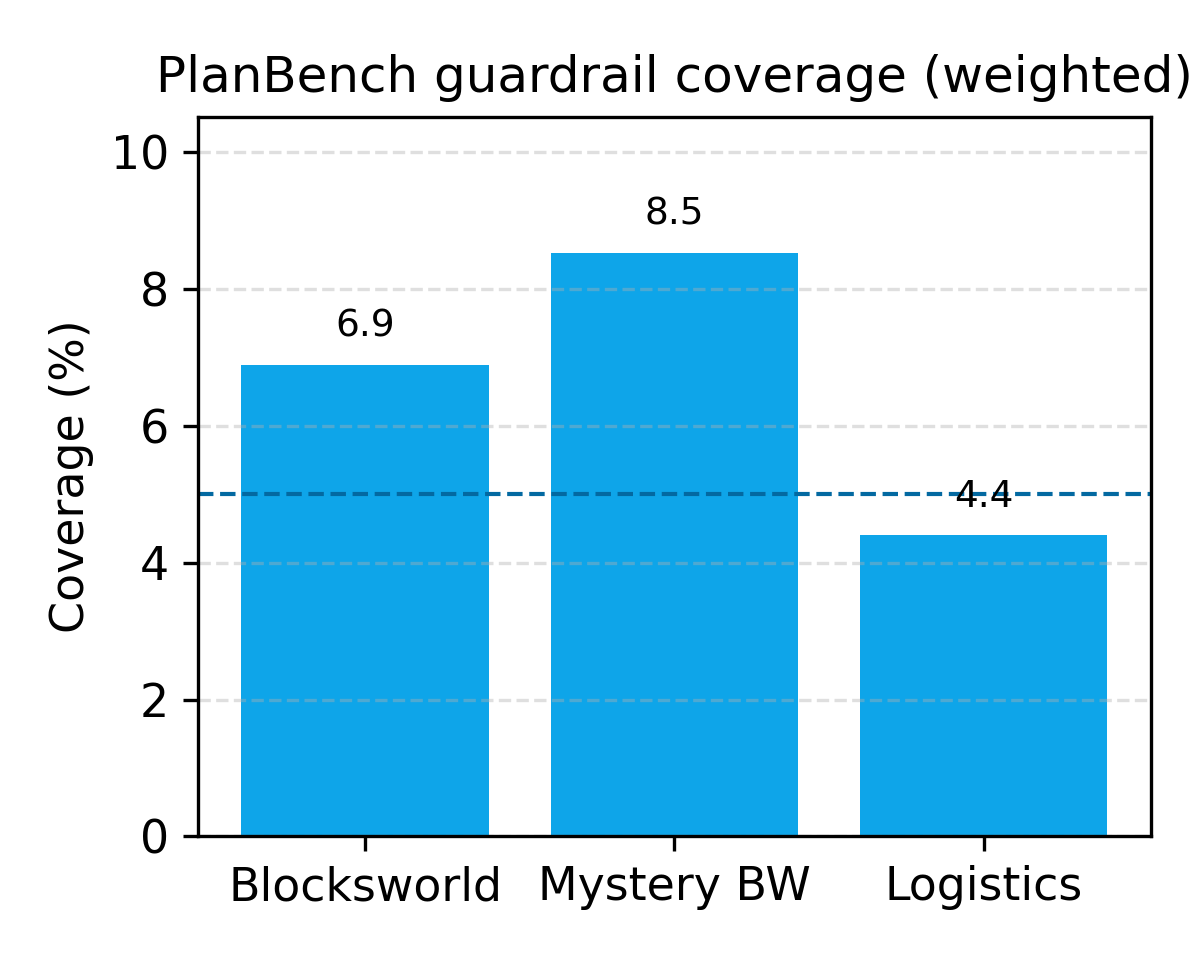
\includegraphics[width=\textwidth]{figures/planbench_guardrail.png}
    \caption{Foreground coverage.}
  \end{subfigure}\hfill
  \begin{subfigure}[t]{0.32\textwidth}
    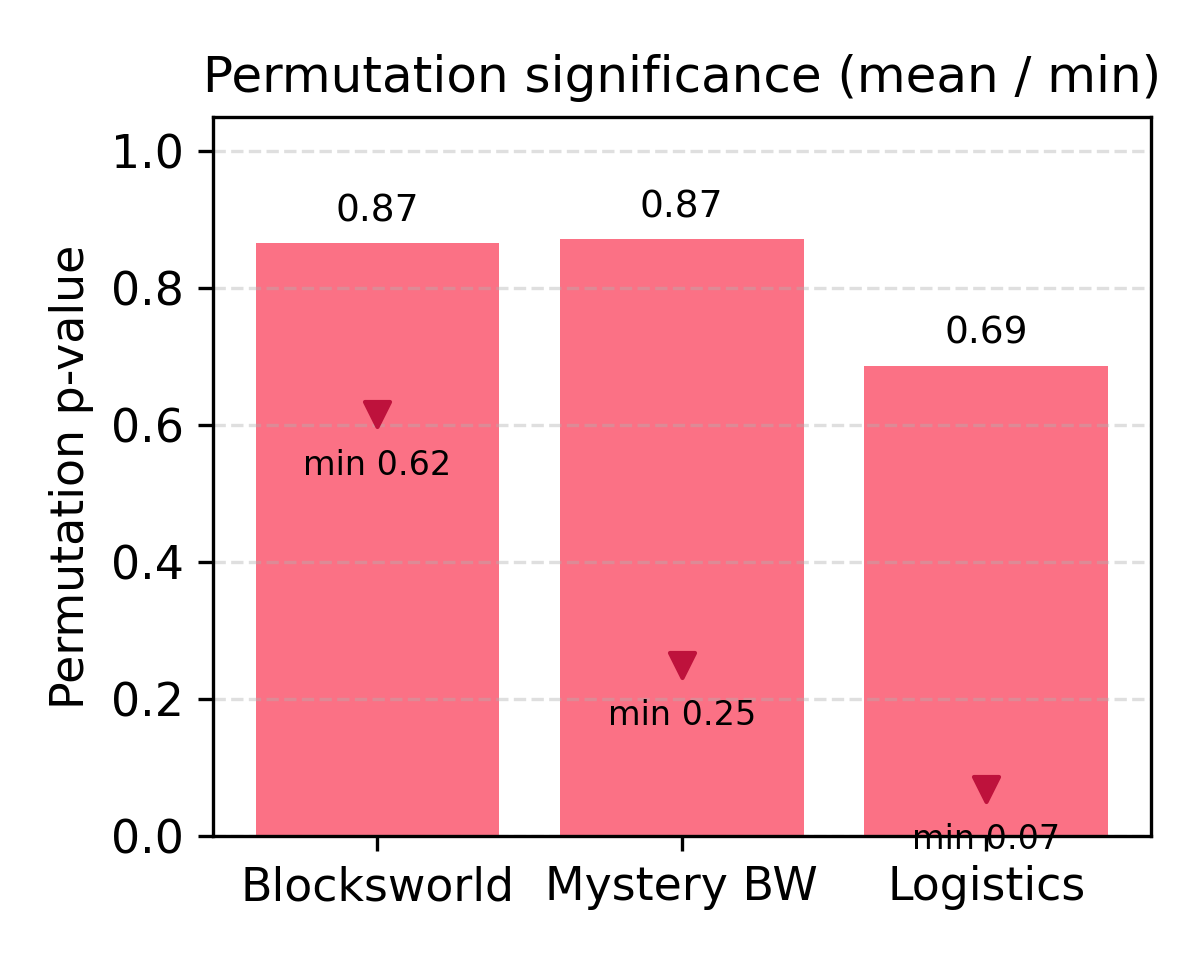
\includegraphics[width=\textwidth]{figures/planbench_permutation.png}
    \caption{Permutation trend.}
  \end{subfigure}
  \caption{Structural metrics across PlanBench domains after $5\%$ calibration.}
  \label{fig:planbench-metrics}
\end{figure}

\subsection{Permutation Significance}
Permutation outcomes appear in Table~\ref{tab:permutation}. Weighted coverage
remains at $4$--$9\%$ across domains, yet permutation $p$-values cluster near
unity, indicating that alert placement is still statistically similar to random
schedules. The lowest observed $p$-value (Logistics, $0.065$) suggests slight
sensitivity, but additional discriminative signals are required for stronger
claims.

\begin{table}[h]
  \centering
  \caption{Permutation statistics using $5{,}000$ iterations. Coverage-weighted is computed over all windows.}
  \label{tab:permutation}
  \begin{tabular}{lcccc}
    \toprule
    Dataset & Coverage-weighted (\%) & Mean lead (steps) & Mean $p$ & Min $p$ \\
    \midrule
    Blocksworld (invalid) & $6.89$ & $4.45$ & $0.87$ & $0.61$ \\
    Mystery BW (invalid) & $8.53$ & $1.76$ & $0.87$ & $0.24$ \\
    Logistics (invalid) & $4.41$ & $2.86$ & $0.69$ & $0.065$ \\
    PlanBench (invalid aggregate) & $5.47$ & $7.59$ & $0.89$ & $0.10$ \\
    \bottomrule
  \end{tabular}
\end{table}

\subsection{Structural Twin Alignment}
Twin recall remains perfect on PlanBench traces across the inspected ANN
thresholds. Figure~\ref{fig:tau-planbench} plots acceptance curves showing $100\%$
recall up to $\tau=0.50$, indicating substantial alignment headroom for future
tightening.

\begin{figure}[h]
  \centering
  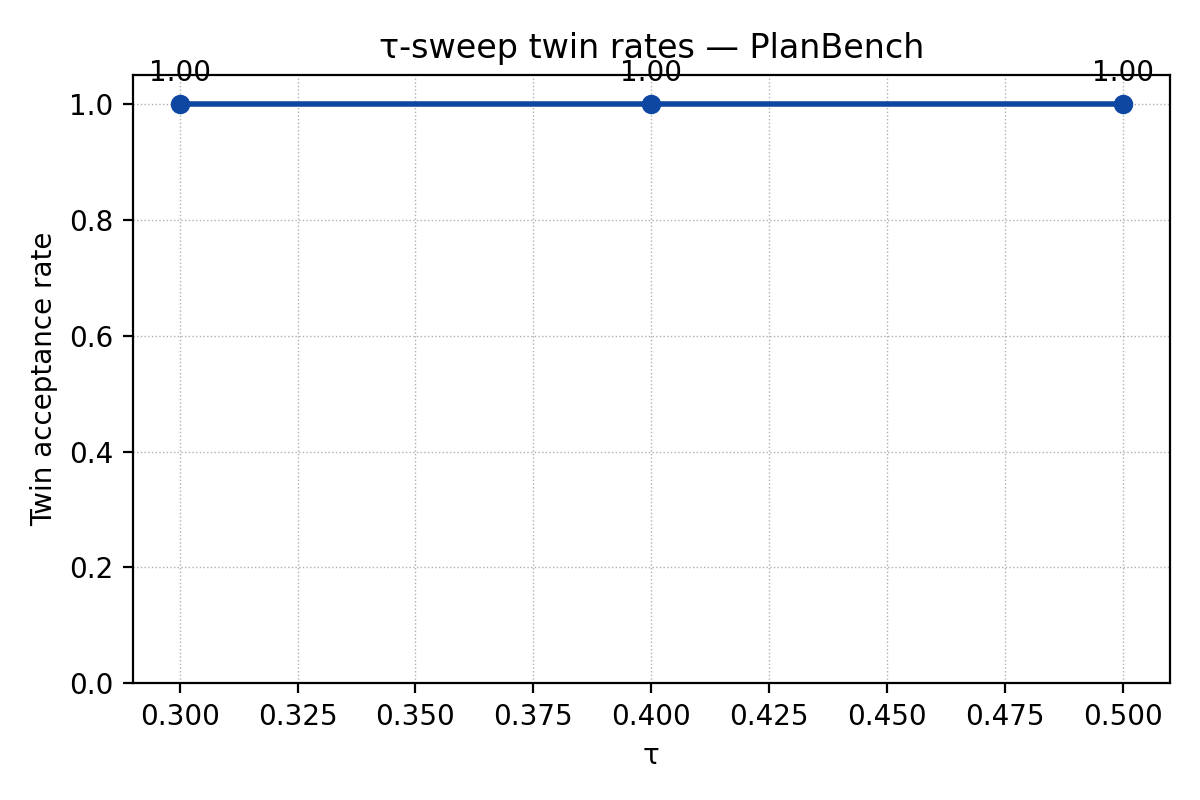
\includegraphics[width=0.78\textwidth]{../note/fig_tau_sweep_planbench.png}
  \caption{PlanBench twin acceptance across ANN thresholds.}
  \label{fig:tau-planbench}
\end{figure}

\subsection{CodeTrace Maintenance Tasks}
We retain the CodeTrace evaluation to illustrate STM behaviour beyond planning.
Table~\ref{tab:codetrace-per-task} summarises the per-task deltas, and
Table~\ref{tab:codetrace-aggregate} reports aggregate statistics. STM reduces
iterations-to-green by roughly $35\%$ while constraining alerts to a single
foreground window per task. These results contextualise the manifold's utility in
software maintenance, complementing symbolic planning benchmarks.

\begin{table}[h]
  \centering
  \caption{Per-task comparison between baseline and STM-assisted CodeTrace runs.}
  \label{tab:codetrace-per-task}
  \begin{tabular}{lcccccc}
    \toprule
    Task & Variant & Steps & Test Runs & Diagnostics & Alerts & Alert Ratio \\
    \midrule
    Flaky retry test & Baseline & 6 & 3 & 0 & 0 & 0.00 \\
                      & STM & 4 & 2 & 0 & 1 & 0.25 \\
    Service rename & Baseline & 8 & 3 & 0 & 0 & 0.00 \\
                   & STM & 5 & 1 & 0 & 1 & 0.20 \\
    Missing import & Baseline & 6 & 0 & 3 & 0 & 0.00 \\
                   & STM & 4 & 0 & 2 & 1 & 0.25 \\
    \bottomrule
  \end{tabular}
\end{table}

\begin{table}[h]
  \centering
  \caption{Aggregate CodeTrace statistics.}
  \label{tab:codetrace-aggregate}
  \begin{tabular}{lcccc}
    \toprule
    Variant & Success Rate & Avg. Steps & Avg. Alert Ratio & Twin Accepts \\
    \midrule
    Baseline & 1.00 & 6.67 & 0.00 & 0 \\
    STM & 1.00 & 4.33 & 0.23 & 3 \\
    \bottomrule
  \end{tabular}
\end{table}

\section{Discussion}
STM guardrails complement instruction-tuned planners by offering calibrated
coverage, actionable lead-time, and structural repair suggestions. The $5\%$
calibration confirms that dense percentile sweeps can reach low foreground
budgets without degrading twin recall. However, high permutation $p$-values
suggest the current metrics remain weakly discriminative. This observation aligns
with the caution noted in planning-focused instruction tuning \cite{verma2025pddlinstruct}:
robust plan verification still requires richer signals or domain-specific
reasoning.

\section{Limitations and Future Work}
Two limitations dominate our findings. First, statistical significance remains
weak despite the tighter guardrail; permutations frequently match observed
alerts. Second, adapters currently target PDDL and Python traces, limiting
coverage. Future work will: (i) expand the trace corpus (PlanBench extensions,
CodeTrace telemetry, robotics logs) to explore alternative metrics; (ii) integrate
permutation-aware objective functions during calibration; and (iii) formalise the
link between STM alerts and logical reasoning traces used in instruction-tuned
models.

\section{Conclusion}
We provide a research-focused account of STM guardrails for symbolic planning
agents, delivering calibrated configurations, permutation analyses, and
reproducible scripts. The release surfaces a clear agenda: maintain low alert
budgets while strengthening statistical significance and broadening adapter
coverage. We hope this baseline informs future collaboration with the PlanBench
community and complementary instruction-tuning efforts.

\appendix

\section{Reproducibility Checklist}
Key commands are listed below; outputs are referenced throughout the text and in
\texttt{docs/tests/}.

\begin{lstlisting}[style=stm]
# Export STM states per domain
for dom in blocksworld mystery_bw logistics; do
  .venv/bin/python scripts/planbench_to_stm.py \
    --input-root data/planbench_public \
    --domains $dom \
    --output output/planbench_by_domain/$dom \
    --window-bytes 256 --stride 128 \
    --path-threshold 0.10 --signal-threshold 0.10 \
    --twin-distance 0.40 --twin-top-k 3 --verbose
done

# Calibrate router guardrails (Listing~\ref{lst:calibration})
# Permutation analysis
for dom in blocksworld mystery_bw logistics; do
  .venv/bin/python scripts/run_permutation_guardrail.py \
    output/planbench_by_domain/$dom \
    analysis/router_config_${dom}_invalid_5pct.json \
    --iterations 5000 \
    --output docs/tests/permutation_${dom}_5pct.json
done

.venv/bin/python scripts/run_permutation_guardrail.py \
  output/planbench_public \
  analysis/router_config_invalid_5pct.json \
  --iterations 5000 \
  --output docs/tests/permutation_planbench_invalid_5pct.json

# Regression tests
.venv/bin/pytest  # 17 passed, 1 skipped
\end{lstlisting}

\begin{thebibliography}{9}
\bibitem{planbench} E. Gripper, L. Pineda, and P. Shah. \emph{PlanBench: A Benchmark Suite for Plan Validation}. MIT CSAIL Technical Report, 2023.
\bibitem{stm-manifold} SepDynamics Research. \emph{Structural Manifold Methods for Early Warning}. Internal Whitepaper, 2024.
\bibitem{verma2025pddlinstruct} P. Verma, N. La, A. Favier, S. Mishra, and J. A. Shah. \emph{Teaching LLMs to Plan: Logical Chain-of-Thought Instruction Tuning for Symbolic Planning}. arXiv:2509.13351, 2025.
\end{thebibliography}

\end{document}
